%!TEX root = ../thesis.tex

\section{本章の概要}

本章では,2章で述べたようにロボットの行動を考慮した歩行者の軌道予測を行う手法を提案する.学習に用いたアルゴリズムに関する内容を3.2章,

% 以下では,予測を行うネットワーク構造とその学習方法に関して説明する.

% 〜について目指す.〜について提案する.

\section{問題設定}
本論文における歩行者のグラフ表現を説明する.時刻$t$におけるシーン内の歩行者の位置を表す空間グラフを$G_t = (V_t, E_t)$と定義する.ここで,$V_t = \{ v^i_t \mid i = 1, \dots N \}$はグラフ$G_t$のノードの集合であり,各ノード$v^i_t$は$i$番目の歩行者の位置$(x^i_t, y^i_t)$を属性として持つ.$E_t = \{ e^{ij}_t \mid i, j = 1, \dots N \}$はグラフ$G_t$のエッジの集合であり,$e^{ij}_t$はノード$v^i_t$と$v^j_t$が接続されている場合1,そうでない場合0の値をとる.

人間の軌道予測は,歩行者の将来の2次元空間の$x,y$座標を,事前観測の情報を与えて予測ステップ分出力することである.
ここで,歩行者$i$の各時刻の位置を
\begin{equation}
  V_t = \{ v^i_t = (x^i_t, y^i_t) \in \mathbb{R}^2 \mid i = 1, \dots N \}
\end{equation}
と表す.また,$t_{obs}$を観測時間としたとき,観測された全歩行者の位置データを
\begin{equation}
  V_{obs} = \{ V_t \mid t = 1, \dots t_{obs} \}  
\end{equation}
と表す.ここで,時刻$t$の2次元空間における歩行者$i$の位置の確率分布を
\begin{equation}
  \hat{V}_t = \{ \hat{p}^i_t = (\hat{x}^i_t, \hat{y}^i_t) \mid i = 1, \dots N \} \label{hat-pos}
\end{equation}
と表す.$t_{pred}$を予測時間としたとき,予測する全歩行者の位置データを
\begin{equation}
  V_{pred} = \{ \hat{V}_t \mid t = t_{obs + 1}, \dots t_{pred} \}
\end{equation}
と表すことができる.$p^i_t$が$\mathcal{N}(\mu^i_t, \sigma^i_t, \rho^i_t)$となる2変量ガウス分布に従うと仮定する.すなわち,$\hat{p}^i_t$は平均$\hat{\mu}^i_t$,分散$\hat{\sigma}^i_t$,相関係数$\hat{\rho}^i_t$を持つガウス分布
\begin{equation}
  \hat{p}^i_t \sim \mathcal{N}(\hat{\mu}^i_t, \hat{\sigma}^i_t, \hat{\rho}^i_t)
\end{equation}
に従う.ここで,平均を$\hat{\mu}^i_t = (\hat{\mu}^i_{x, t}, \hat{\mu}^i_{y, t})$,分散を$\hat{\sigma}^i_t = (\hat{\sigma}^i_{x, t}, \hat{\sigma}^i_{y, t})$とする.

\section{ネットワーク構造}
本手法で用いられるネットワークは,エンコーダ・デコーダ構造で構成されている.ネットワークは,主にエンコーダモジュール,グラフアテンションネットワークモジュール,デコーダモジュールから構成される.エンコーダモジュールでは,入力データから特徴量を抽出し,グラフアテンションネットワークを用いて,ノード間の関係性を学習する.これらの潜在表現を基に,デコーダモジュールで目的のシーケンス長の予測を行う.
\figref{Fig:network}は,このネットワークの概要を表している.

\begin{figure}[hbtp]
  \centering
 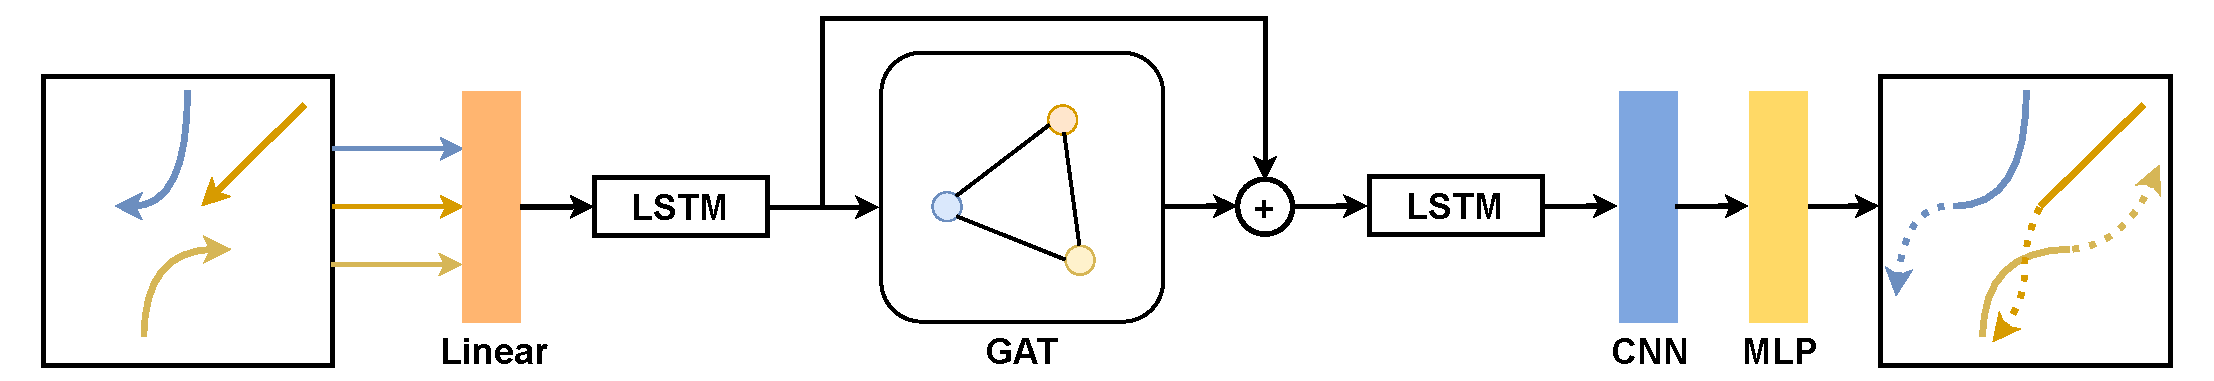
\includegraphics[keepaspectratio, scale=0.36]
      {images/network-comp.pdf}
 \caption{Network Structure}
 \label{Fig:network}
\end{figure}   

\subsection{エンコーダモジュール}
エンコーダでは,まず,入力の各時刻における歩行者の過去の位置は,線形変換層$\phi_{emb}$を用いて高次元空間に埋め込まれる.この埋め込み表現は,LSTM層に入力され,歩行者の過去の位置情報を時間的に処理し,隠れ状態を出力する.隠れ状態は,歩行者の過去の動きを要約したものであり,次のグラフアテンションネットワークに渡される.エンコーダでの処理を式\eqref{emb},\eqref{lstm-en}に示す.なお,$v^i_t \text{と} v^t_i$は等価である.
\begin{align}
  e^t_i &= \phi_{emb}(v^t_i ; W_{emb}) \label{emb} \\
  h_i &= \text{LSTM}_{en}(e^t_i, h^{t-1}_i ; W_{en}) \label{lstm-en}
\end{align}

\subsection{グラフアテンションネットワーク}
ネットワークの中核を担うグラフアテンションネットワーク(GAT)\cite{velickovic2017graph-gat}は,複数層で構成される.各GAT層は,マルチヘッドアテンション機構を用いて,各ノードの特徴をその近傍ノードの特徴と集約する.アテンション機構は,ノード間の関係の強さに基づいて重み付けを行うため,より関連性の高いノードからの情報が強調される.本ネットワークでは,複数のGAT層を積み重ねることで,グラフ構造における高次の依存関係を捉えることができる.各タイムステップにおいて,対応する隣接行列を用いてグラフ畳み込みが実行され,動的なグラフ構造の変化にも対応できる.

歩行者$i$の隠れ状態$h_i$が与えられたとき,全ての歩行者に対して,複数のGAT層を適用する.各層は以下のように適用される.式\eqref{gat-eij}は,ノード$i$に対するノード$j$の特徴の重要度を表している.$W$は重み行列であり,$a$は共有アテンション機構である.また,$\sigma$は活性化関数であり,本手法ではPReLU\cite{he2015delving-prelu}を用いた.
\begin{align}
  e_{ij} = a(Wh_i, Wh_j) \label{gat-eij} \\
  \alpha_{ij} = \text{softmax}_{j}(e_{ij}) \\
  h'_i = \sigma\Bigg(\sum_{j \in \mathcal{N}_i} \alpha_{ij}Wh_j \Bigg)
\end{align}

\subsection{デコーダモジュール}
GAT層からの出力は,デコーダモジュールによって将来の歩行者の予測位置に変換される.まず,2つ目のLSTM層がGATによって生成された時空間特徴表現をさらに時間的に処理する.次に,1次元畳み込み層を用いて,入力シーケンス長から予測シーケンス長への変換が行われる.この層は,予測時間に合わせて特徴表現を調整する役割を果たす.最後に多層パーセプトロン(MLP)が予測値を生成する.式\eqref{output}のように,ネットワークの最終的な出力は5次元である.なお,$\hat{P}^t_i\text{と}\hat{P}^i_t$は等価である.
\begin{align}
  h''_i = \text{LSTM}_{dec}(h'_i, h_{deci}; W_{dec})\\
  c^t_i = \text{CNN}(h''_i; W_{cnn}) \\
  \hat{P}^t_i = \text{MLP}_{d}(c^t_i; W_{d}) \\
  \hat{P}^i_t = [\hat{\mu}^i_{x,t}, \hat{\mu}^i_{y, t}, \hat{\sigma}^i_{x, t}, \hat{\sigma}^i_{y, t}, \hat{\rho}^i_t] \label{output}
\end{align}

さらに,本ネットワークでは\figref{Fig:network}のように,GAT層とLSTM層の出力にスキップ接続\cite{he2016deep-resnet}を導入することで,勾配消失問題\cite{hochreiter2001gradient-grad,weinleindiplomarbeit-grad, schmidhuber2015deep-grad}を軽減し,学習を安定化させる.このアーキテクチャにより,時系列データの動的な変化とグラフ構造におけるノード間の複雑な関係を効果的に捉え,高精度な予測を実現する.

\section{データセットと評価指標}

\section{学習方法}

\section{ロボットの行動を考慮した軌道予測}

\section{設計したネットワークの予備実験}

\subsection{実験方法}
\subsection{結果}
\subsection{考察}

\newpage
